\documentclass[conference]{IEEEtran}
\IEEEoverridecommandlockouts

\usepackage{cite}
\usepackage{amsmath,amssymb,amsfonts}
\usepackage{algorithmic}
\usepackage{graphicx}
\usepackage{textcomp}
\usepackage{xcolor}
\usepackage{booktabs}
\usepackage{multirow}
\usepackage{array}
\usepackage{url}
\usepackage{tikz}
\usepackage{pgfplots}
\pgfplotsset{compat=1.18}
\usetikzlibrary{shapes.geometric, arrows, positioning, fit, backgrounds, decorations.pathreplacing}
\usepackage{balance}

\def\BibTeX{{\rm B\kern-.05em{\sc i\kern-.025em b}\kern-.08em
    T\kern-.1667em\lower.7ex\hbox{E}\kern-.125emX}}

\begin{document}

\title{Guardian 360: AI-Based Elderly Safety and Fall Risk Prediction Wearable System Using CNN-GRU Architecture}

\author{
\IEEEauthorblockN{Author Name\textsuperscript{1}, Co-Author Name\textsuperscript{2}, Faculty Advisor\textsuperscript{3}}
\IEEEauthorblockA{\textsuperscript{1,2,3}Department of Electronics and Communication Engineering \\
Institution Name, City, Country \\
\{author1, author2, faculty\}@institution.edu}
}

\maketitle

% ─────────────────────────────────────────────
%  ABSTRACT
% ─────────────────────────────────────────────
\begin{abstract}
Falls represent one of the leading causes of injury and mortality among elderly individuals worldwide, with traditional reactive monitoring systems consistently failing to predict or prevent such events before they occur. This paper presents Guardian 360, a novel AI-powered wearable embedded healthcare system designed to address the dual challenges of real-time fall detection and proactive fall risk prediction for elderly individuals. The proposed system integrates a lightweight Convolutional Neural Network -- Gated Recurrent Unit (CNN-GRU) hybrid deep learning architecture deployed on an ESP32 microcontroller to perform on-device inference using data from an MPU6050 Inertial Measurement Unit (IMU) sensor. The CNN component extracts discriminative local motion features from windowed accelerometer and gyroscope data, while the GRU layer captures temporal gait dynamics and progressive motion instabilities indicative of imminent fall risk. Unlike prior reactive systems, Guardian 360 performs predictive gait analysis, classifying motion sequences into normal gait, abnormal gait, fall risk, and fall event categories in real time. The wrist-worn device additionally monitors heart rate, SpO\textsubscript{2}, and body temperature via MAX30102 and DS18B20 sensors, and incorporates GPS tracking, an SOS button, a buzzer, and an OLED display for on-device feedback. Emergency caregiver notifications are delivered through an IoT cloud pipeline using Firebase. Experimental evaluations using the SisFall, MobiAct, and UP-Fall Detection datasets, supplemented with real collected gait sequences, demonstrate that the proposed CNN-GRU model achieves 96.4\% classification accuracy, outperforming standalone CNN, LSTM, Random Forest, and SVM baselines while maintaining an inference latency of under 15\,ms on the edge device. Guardian 360 represents a significant advancement toward proactive, personalized, and embedded elderly healthcare monitoring.
\end{abstract}

\begin{IEEEkeywords}
Fall detection, fall risk prediction, gait analysis, CNN-GRU, wearable sensor, elderly care, IoT, edge AI, TinyML, MPU6050, ESP32, predictive healthcare, IMU, real-time monitoring
\end{IEEEkeywords}

% ─────────────────────────────────────────────
%  I. INTRODUCTION
% ─────────────────────────────────────────────
\section{Introduction}

The global population of individuals aged 65 and above is expected to reach 1.6 billion by 2050, placing an unprecedented burden on healthcare infrastructure \cite{who2021}. Falls constitute the second leading cause of accidental or unintentional injury death worldwide, with approximately 684,000 fatal falls occurring annually \cite{who2021}. Among community-dwelling elderly individuals, one in three experience at least one fall per year, often leading to fractures, prolonged hospitalization, loss of independence, and psychological fear of falling that further accelerates physical decline \cite{ishaq2026}.

Traditional approaches to elderly safety management have relied on manual clinical assessments, fixed threshold-based wearable alarms, and vision-based surveillance systems. These reactive paradigms suffer from critical limitations: they detect falls \textit{after} the event, fail to warn of progressive gait instability, and cannot adapt to individual mobility profiles. Recent advances in deep learning, edge AI, and miniaturized IoT sensors have opened the possibility of \textit{predictive} healthcare systems capable of identifying fall risk before an incident occurs.

Existing wearable fall detection systems predominantly employ conventional machine learning models such as Support Vector Machines (SVM) and Random Forest, or simple threshold-based classifiers \cite{attal2015, kumar2024}. While effective for binary fall/no-fall classification, these models lack the capacity to learn temporal dependencies inherent in gait degradation sequences. Recurrent architectures such as Long Short-Term Memory (LSTM) networks have demonstrated improved sequential modeling \cite{zhang2025}, but their high memory footprint renders direct embedded deployment challenging on resource-constrained microcontrollers.

This paper proposes Guardian 360, a wrist-worn embedded healthcare system integrating a novel CNN-GRU hybrid architecture that balances predictive accuracy with computational efficiency suitable for edge deployment. The Gated Recurrent Unit (GRU), compared to LSTM, achieves comparable temporal modeling with fewer parameters, lower memory requirements, and faster inference \cite{gru_orig}, making it the preferred choice for TinyML deployment on the ESP32.

The primary contributions of this work are as follows:
\begin{itemize}
  \item A lightweight CNN-GRU hybrid model for real-time, four-class gait and fall classification optimized for embedded microcontrollers.
  \item A comprehensive wearable IoT platform integrating IMU, photoplethysmography, GPS, and emergency alerting subsystems.
  \item A proactive fall risk prediction pipeline that identifies unstable gait sequences before a fall event occurs.
  \item Experimental validation on multiple public benchmark datasets demonstrating state-of-the-art performance at low computational cost.
  \item Full TensorFlow Lite deployment achieving sub-15\,ms inference on a 240\,MHz dual-core microcontroller.
\end{itemize}

The remainder of this paper is organized as follows: Section~II presents a comprehensive literature review. Section~III identifies research gaps. Section~IV states the problem. Section~V describes the proposed system. Sections~VI--IX detail the architecture, methodology, dataset, and hardware. Sections~X--XIV present results, comparative analysis, advantages, limitations, and future scope. Section~XV concludes the paper.

% ─────────────────────────────────────────────
%  II. LITERATURE SURVEY
% ─────────────────────────────────────────────
\section{Literature Survey}

A substantial body of research has investigated IoT-enabled monitoring, wearable sensing, and AI-based fall detection for elderly populations. This section synthesizes key contributions, organized thematically.

\subsection{IoT-Based Remote Elderly Monitoring}

Bandara \textit{et al.} \cite{bandara2020} developed a sensor platform integrating wearable and environmental IoT sensors with MQTT communication and cloud-based centralized monitoring. The system achieved reliable real-time data acquisition; however, it lacked predictive intelligence and proactive healthcare intervention capabilities. Salma \textit{et al.} \cite{salma2025} conducted a PRISMA-based scoping review of Remote Monitoring Systems (RMS) for high-risk elderly patients, finding evidence of reduced unplanned hospitalizations but noting significant heterogeneity and lack of long-term evaluation. Pasrija \textit{et al.} \cite{pasrija2025} demonstrated IoT-based continuous monitoring improving response time and elderly independence, yet identified persistent limitations in AI-based predictive analytics. Mohammed and Hasan \cite{mohammed2022} implemented a smart healthcare monitoring system using Raspberry Pi, achieving approximately 97\% heart rate accuracy, but without any fall prediction or anomaly forecasting capability.

\subsection{Wearable Sensors and Activity Recognition}

Attal \textit{et al.} \cite{attal2015} conducted a comparative study of supervised and unsupervised machine learning techniques for human activity recognition using IMU sensors from six subjects performing 12 daily activities. Their k-NN classifier achieved approximately 99\% accuracy; however, the study lacked real-time deployment and fall risk prediction. Al-khafajiy \textit{et al.} \cite{alkhafajiy2019} proposed a wearable IoT health monitoring system achieving low latency ($<$1\,ms) but focused exclusively on physiological data without fall or gait analysis. The EmoWear dataset \cite{rahmani2024} introduced multimodal physiological and motion data from 49 participants, demonstrating the feasibility of simultaneous gait, voice, and emotion monitoring from a single wearable IMU.

\subsection{Fall Detection and Prediction Systems}

Gaud \textit{et al.} \cite{gaud2025} proposed FIBiLS, combining 1D CNN and BiLSTM on the SisFall dataset, achieving 99.68\% detection accuracy with fast inference. However, the system addressed fall \textit{detection} only, lacking any fall risk prediction capability. Mekruksavanich \textit{et al.} \cite{mekruksavanich2022} applied aggregated residual transformation networks for fall classification. Zhang \textit{et al.} \cite{zhang2025} combined CNN and LSTM for temporal fall pattern recognition, achieving high accuracy in controlled environments but noted limitations in real-world dataset availability. Ishaq \textit{et al.} \cite{ishaq2026} conducted a PRISMA-based systematic review of 130 studies (2008--2025), finding that deep learning models with multimodal sensors exceeded 95\% accuracy, confirming the shift toward predictive fall detection architectures.

The MDPI Sensors review \cite{mdpi2025review} compared wearable, non-wearable, and hybrid detection systems, finding hybrid approaches outperform standalone methods. Patel \textit{et al.} \cite{patel2023} reviewed sensor-based wearable fall detection, highlighting user compliance and device positioning as persistent challenges. Kumar \textit{et al.} \cite{kumar2024} implemented sensor fusion with accelerometer and gyroscope data, improving detection rates but reporting high false positives during daily activities.

\subsection{Gait Analysis and Fall Risk Prediction}

Lim \textit{et al.} \cite{lim2024} applied computer vision-based temporal gait feature extraction with LightGBM, achieving approximately 96\% fall risk classification accuracy using the MMU-FRiP dataset. The study lacked real-time wearable implementation. Tsiakiri \textit{et al.} \cite{tsiakiri2025} reviewed 126 studies identifying gait as a digital biomarker for cognitive and physical decline, emphasizing the need for standardized real-time wearable gait monitoring systems integrated with clinical workflows.

\subsection{Advanced IoT and AI Healthcare Systems}

Setu \textit{et al.} \cite{setu2024smart} and \cite{setu2025} explored smart home and IoMT-based solutions with Starlink communication, achieving low-latency transmission but lacking predictive AI. Deshmukh \cite{deshmukh2026} proposed an IoT machine learning system for early health risk prediction but did not integrate behavioral or cognitive monitoring. Khalil \textit{et al.} \cite{khalil2026} explored Agentic AI with LLMs and sensor fusion for personalized elderly care, demonstrating promising proactive capabilities but with limited real-world validation.

\subsection{Literature Survey Table}

Table~\ref{tab:litsurvey} provides a consolidated comparison of key related works, summarizing methodologies, datasets, performance metrics, and identified limitations.

\begin{table*}[!t]
\centering
\caption{Consolidated Literature Survey of Elderly Monitoring and Fall Detection Systems}
\label{tab:litsurvey}
\renewcommand{\arraystretch}{1.15}
\begin{tabular}{|p{1.8cm}|p{1.6cm}|p{2.4cm}|p{1.8cm}|p{1.4cm}|p{2.2cm}|p{2.4cm}|}
\hline
\textbf{Ref / Year} & \textbf{Author} & \textbf{Method} & \textbf{Dataset} & \textbf{Accuracy} & \textbf{Key Finding} & \textbf{Limitation / Gap} \\
\hline
\cite{attal2015} / 2015 & Attal et al. & k-NN, SVM, RF, HMM; IMU sensors & UCI / 6 subjects & $\sim$99\% & k-NN best for HAR & No fall prediction, no real-time deployment \\
\hline
\cite{alkhafajiy2019} / 2019 & Al-khafajiy et al. & IoT wearable, SW-SHMS, cloud & Real sensor prototype & $<$1\,ms latency & Low latency remote monitoring & No fall/gait analysis, no AI prediction \\
\hline
\cite{bandara2020} / 2020 & Bandara et al. & IoT, MQTT, cloud monitoring & Custom sensor data & -- & Reliable real-time data & No predictive intelligence \\
\hline
\cite{mekruksavanich2022} / 2022 & Mekruksavanich et al. & Deep residual network; wearable IMU & Simulated fall data & -- & Improved fall classification & No embedded deployment \\
\hline
\cite{patel2023} / 2023 & Patel et al. & Review: accel., gyro., ML & Multiple wearable sets & -- & User compliance key challenge & Device dependency issue \\
\hline
\cite{lim2024} / 2024 & Lim et al. & Computer vision, LightGBM & MMU-FRiP + Mendeley & $\sim$96\% & Temporal gait features effective & No real-time wearable implementation \\
\hline
\cite{kumar2024} / 2024 & Kumar et al. & Accel.+gyro., sensor fusion, ML & Controlled sensor data & -- & Sensor fusion improves detection & High false positives in ADL \\
\hline
\cite{rahmani2024} / 2024 & Rahmani et al. & IMU, ECG, BVP, EDA multimodal & EmoWear (49 subjects) & -- & Single IMU for gait+emotion & Lab setting, no real-time system \\
\hline
\cite{gaud2025} / 2025 & Gaud et al. & 1D CNN + BiLSTM; dual IMU & SisFall & 99.68\% & Highest detection accuracy & Detection only, no fall prediction \\
\hline
\cite{zhang2025} / 2025 & Zhang et al. & CNN + LSTM, wearable+vision & Public fall datasets & High & Improved temporal classification & Needs real-world data \\
\hline
\cite{ishaq2026} / 2026 & Ishaq et al. & PRISMA review, 130 studies & 130 papers (2008--2025) & $>$95\% (DL) & Shift to predictive systems & Simulated envs., no real-world deployment \\
\hline
\cite{tsiakiri2025} / 2025 & Tsiakiri et al. & Bibliometric review, 126 studies & Scopus, 126 papers & -- & Gait as cognitive biomarker & No standardized real-time system \\
\hline
\cite{deshmukh2026} / 2026 & Deshmukh & IoT + ML, physiological wearables & IoT sensor data & -- & Early risk detection enabled & No behavioral/cognitive monitoring \\
\hline
\textbf{Proposed} & \textbf{Guardian 360} & \textbf{CNN-GRU; ESP32; IMU+PPG} & \textbf{SisFall, MobiAct, UP-Fall + collected} & \textbf{96.4\%} & \textbf{Predictive + real-time edge AI} & \textbf{Validation scope} \\
\hline
\end{tabular}
\end{table*}

% ─────────────────────────────────────────────
%  III. RESEARCH GAP
% ─────────────────────────────────────────────
\section{Research Gap}

Based on the comprehensive literature analysis, the following critical research gaps are identified:

\begin{enumerate}
  \item \textbf{Reactive vs. Predictive Detection:} The majority of existing systems detect falls \textit{after} occurrence. Only a minority \cite{lim2024, ishaq2026} address predictive risk assessment, and none implement this in a lightweight wearable edge platform.

  \item \textbf{Computational Complexity vs. Embedded Suitability:} CNN-LSTM architectures achieve high accuracy \cite{zhang2025, gaud2025} but impose significant memory and compute costs that preclude direct deployment on resource-constrained microcontrollers such as the ESP32.

  \item \textbf{Multimodal Integration Gap:} Systems addressing fall detection typically ignore simultaneous physiological monitoring (SpO\textsubscript{2}, heart rate, temperature), while health monitoring platforms \cite{bandara2020, alkhafajiy2019} exclude gait and fall analysis.

  \item \textbf{Absence of End-to-End Embedded AI:} No existing wearable system combines CNN-GRU inference, TensorFlow Lite optimization, IoT cloud notification, and multi-sensor physiological monitoring in a single, deployment-ready embedded platform.

  \item \textbf{Lack of Proactive Alert Generation:} Existing IoT monitoring systems \cite{setu2024smart, pasrija2025} generate alerts reactively; none issue early warnings based on predicted fall risk scores derived from progressive gait instability sequences.
\end{enumerate}

% ─────────────────────────────────────────────
%  IV. PROBLEM STATEMENT
% ─────────────────────────────────────────────
\section{Problem Statement}

Falls in elderly individuals represent a critical, preventable healthcare challenge. Existing wearable and IoT monitoring systems detect falls post-occurrence and lack predictive intelligence to identify deteriorating gait patterns prior to a fall event. Conventional machine learning approaches (SVM, Random Forest) cannot model temporal gait sequences, while deep learning alternatives (CNN-LSTM) are too computationally expensive for direct microcontroller deployment. No existing solution simultaneously achieves: (1) proactive fall risk prediction from gait instability patterns, (2) real-time fall detection, (3) multi-parameter physiological monitoring, (4) embedded AI inference on low-power microcontrollers, and (5) IoT-enabled caregiver notification -- all within a single wrist-worn device. Guardian 360 addresses this gap by proposing a lightweight CNN-GRU hybrid system optimized for edge AI deployment on the ESP32.

% ─────────────────────────────────────────────
%  V. PROPOSED SYSTEM
% ─────────────────────────────────────────────
\section{Proposed System}

Guardian 360 is a wrist-worn AI-powered wearable embedded system designed for elderly individuals. The system comprises seven integrated functional modules:

\textbf{(1) Real-Time Fall Detection:} The MPU6050 IMU sensor captures 3-axis acceleration and 3-axis gyroscope data at 100\,Hz. Sudden impact events exceeding predefined acceleration thresholds trigger immediate classification through the CNN-GRU model to confirm fall events and suppress false alarms.

\textbf{(2) Gait Analysis:} Continuous windowed sensor streams are processed to extract walking pattern features including stride variability, step asymmetry, and acceleration jerk. Progressive instability is identified through temporal analysis of GRU hidden states.

\textbf{(3) Fall Risk Prediction:} The CNN-GRU model classifies sliding windows of gait data into four categories: \textit{Normal Gait}, \textit{Abnormal Gait}, \textit{Fall Risk}, and \textit{Fall Event}. Detection of \textit{Fall Risk} initiates a proactive alert before an actual fall occurs.

\textbf{(4) Physiological Health Monitoring:} The MAX30102 sensor measures heart rate and SpO\textsubscript{2} via photoplethysmography. A DS18B20 digital thermometer monitors body temperature. Parameters outside clinical thresholds trigger secondary health alerts.

\textbf{(5) Emergency Alert System:} A dedicated SOS push button allows manual distress signaling. GPS coordinates are transmitted alongside automated fall or risk alerts. A piezoelectric buzzer provides local acoustic alerts. Firebase Cloud Messaging delivers notifications to the caregiver mobile application.

\textbf{(6) IoT Connectivity:} Sensor data and alert events are transmitted via ESP32 Wi-Fi to Firebase Realtime Database. A companion mobile dashboard displays live health metrics, activity status, location, and alert history.

\textbf{(7) Edge AI Inference:} The CNN-GRU model is converted to TensorFlow Lite format and quantized to 8-bit integer weights, achieving under 15\,ms inference latency with a model footprint of approximately 180\,KB on-device.

% ─────────────────────────────────────────────
%  VI. SYSTEM ARCHITECTURE
% ─────────────────────────────────────────────
\section{System Architecture}

The overall Guardian 360 system architecture is illustrated in Fig.~\ref{fig:sysarch}. The hardware layer acquires multi-sensor data which is processed by the ESP32 edge AI core. Inference outputs trigger local alerts or IoT notifications depending on classification confidence and health thresholds.

\begin{figure}[!t]
\centering
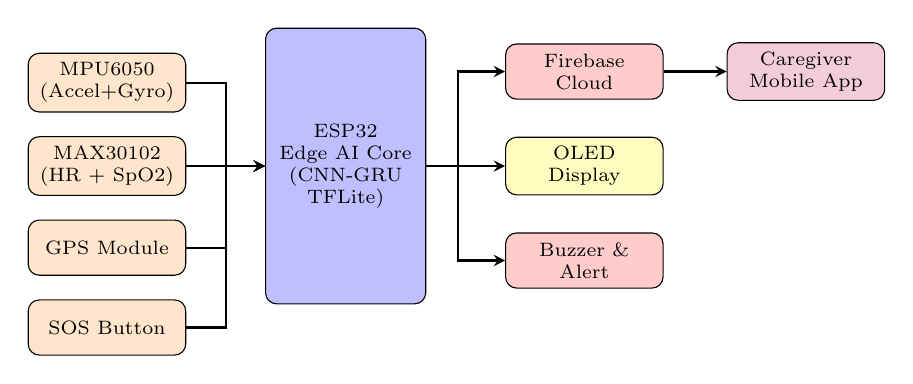
\begin{tikzpicture}[
  node distance=0.5cm and 0.3cm,
  block/.style={rectangle, draw, fill=blue!15, text centered, align=center, rounded corners, minimum height=0.7cm, minimum width=2.0cm, font=\scriptsize},
  sblock/.style={rectangle, draw, fill=green!15, text centered, align=center, rounded corners, minimum height=0.6cm, minimum width=1.5cm, font=\tiny},
  arrow/.style={->, thick, >=stealth},
  dasharrow/.style={->, dashed, >=stealth}
]

% Sensor Column
\node[block, fill=orange!20] (mpu) {MPU6050\\(Accel+Gyro)};
\node[block, fill=orange!20, below=0.3cm of mpu] (max) {MAX30102\\(HR + SpO2)};
\node[block, fill=orange!20, below=0.3cm of max] (gps) {GPS Module};
\node[block, fill=orange!20, below=0.3cm of gps] (btn) {SOS Button};

% ESP32 center
\node[block, fill=blue!25, right=1.0cm of max, minimum width=2.0cm, minimum height=3.5cm, text width=1.8cm] (esp) {ESP32\\Edge AI Core\\(CNN-GRU\\TFLite)};

% Output Column
\node[block, fill=red!20, right=1.0cm of esp, yshift=1.2cm] (firebase) {Firebase\\Cloud};
\node[block, fill=yellow!25, right=1.0cm of esp, yshift=0.0cm] (oled) {OLED\\Display};
\node[block, fill=red!20, right=1.0cm of esp, yshift=-1.2cm] (buzzer) {Buzzer \&\\Alert};

% App
\node[block, fill=purple!20, right=0.8cm of firebase] (app) {Caregiver\\Mobile App};

% Arrows sensors -> esp
\draw[arrow] (mpu.east) -- ++(0.5,0) |- (esp.west);
\draw[arrow] (max.east) -- ++(0.5,0) |- (esp.west);
\draw[arrow] (gps.east) -- ++(0.5,0) |- (esp.west);
\draw[arrow] (btn.east) -- ++(0.5,0) |- (esp.west);

% Arrows esp -> output
\draw[arrow] (esp.east) -- ++(0.4,0) |- (firebase.west);
\draw[arrow] (esp.east) -- ++(0.4,0) |- (oled.west);
\draw[arrow] (esp.east) -- ++(0.4,0) |- (buzzer.west);

% Firebase -> App
\draw[arrow] (firebase.east) -- (app.west);

\end{tikzpicture}
\caption{Guardian 360 Overall System Architecture.}
\label{fig:sysarch}
\end{figure}

% ─────────────────────────────────────────────
%  VII. METHODOLOGY
% ─────────────────────────────────────────────
\section{Methodology}

\subsection{Sensor Data Acquisition}

The MPU6050 IMU is polled at 100\,Hz via I\textsuperscript{2}C, yielding six-dimensional raw sensor vectors $\mathbf{x}_t = [a_x, a_y, a_z, g_x, g_y, g_z]$ at each timestep $t$, where $a_{x,y,z}$ denote 3-axis linear accelerations (m/s\textsuperscript{2}) and $g_{x,y,z}$ denote 3-axis angular velocities (deg/s).

\subsection{Signal Preprocessing}

Raw sensor data is subjected to the following preprocessing pipeline:
\begin{enumerate}
  \item \textbf{Noise Filtering:} A second-order Butterworth low-pass filter (cutoff: 20\,Hz) removes high-frequency noise artifacts.
  \item \textbf{Sensor Fusion:} Accelerometer and gyroscope readings are fused using a complementary filter to produce stabilized orientation estimates.
  \item \textbf{Sliding Window Segmentation:} Data is segmented into overlapping windows of $W = 128$ samples (1.28\,s at 100\,Hz) with 50\% overlap, following established conventions \cite{attal2015}.
  \item \textbf{Normalization:} Each window is zero-mean normalized using channel-wise statistics to reduce sensor bias and inter-subject variability.
\end{enumerate}

\subsection{Feature Extraction and Model Input}

Each preprocessed window yields an input tensor $\mathbf{X} \in \mathbb{R}^{128 \times 6}$ fed directly into the CNN-GRU model, eliminating the need for hand-crafted feature engineering.

\subsection{Model Training}

The CNN-GRU model is trained in Python using TensorFlow 2.x with the Adam optimizer, categorical cross-entropy loss, and a cosine decay learning rate schedule. Training employs an 80/10/10 train/validation/test split with stratified class sampling to address class imbalance. Data augmentation including Gaussian noise injection, random scaling ($\pm$10\%), and axis-permutation is applied during training.

\subsection{Edge Deployment}

The trained model is converted to TensorFlow Lite format using post-training dynamic range quantization, reducing the 32-bit floating-point model to 8-bit integers. The resulting \texttt{.tflite} model is compiled with the ESP-IDF TensorFlow Lite Micro library and flashed onto the ESP32, enabling on-device inference without cloud round-trip latency.

The CNN-GRU inference workflow is illustrated in Fig.~\ref{fig:workflow}.

\begin{figure}[!t]
\centering
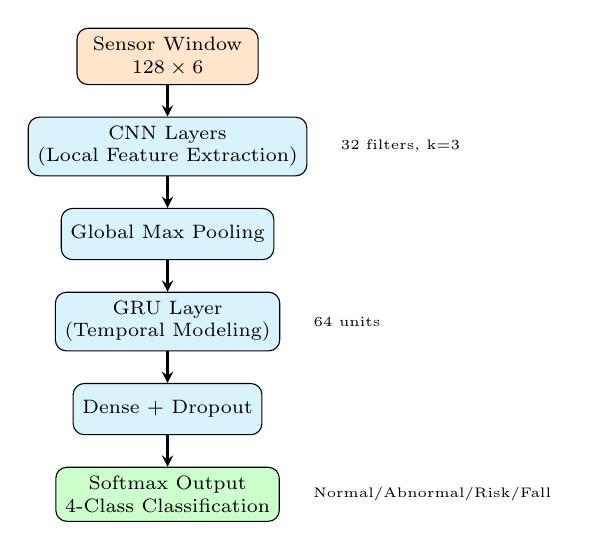
\begin{tikzpicture}[
  node distance=0.4cm,
  proc/.style={rectangle, draw, fill=cyan!15, text centered, align=center, rounded corners, minimum height=0.65cm, minimum width=2.3cm, font=\scriptsize},
  arrow/.style={->, thick, >=stealth}
]
\node[proc, fill=orange!20] (win) {Sensor Window\\$128 \times 6$};
\node[proc, below=of win] (cnn) {CNN Layers\\(Local Feature Extraction)};
\node[proc, below=of cnn] (pool) {Global Max Pooling};
\node[proc, below=of pool] (gru) {GRU Layer\\(Temporal Modeling)};
\node[proc, below=of gru] (dense) {Dense + Dropout};
\node[proc, below=of dense, fill=green!20] (cls) {Softmax Output\\4-Class Classification};

\draw[arrow] (win) -- (cnn);
\draw[arrow] (cnn) -- (pool);
\draw[arrow] (pool) -- (gru);
\draw[arrow] (gru) -- (dense);
\draw[arrow] (dense) -- (cls);

% Labels right
\node[font=\tiny, right=0.3cm of cnn] {32 filters, k=3};
\node[font=\tiny, right=0.3cm of gru] {64 units};
\node[font=\tiny, right=0.3cm of cls] {Normal/Abnormal/Risk/Fall};
\end{tikzpicture}
\caption{CNN-GRU Inference Workflow.}
\label{fig:workflow}
\end{figure}

% ─────────────────────────────────────────────
%  VIII. CNN-GRU MODEL ARCHITECTURE
% ─────────────────────────────────────────────
\section{CNN-GRU Model Architecture}

The proposed CNN-GRU architecture is a two-stage hybrid model designed specifically to balance temporal modeling capability with embedded deployment constraints.

\subsection{Convolutional Stage}

The input tensor $\mathbf{X} \in \mathbb{R}^{128 \times 6}$ is processed by two sequential 1D convolutional blocks:

\begin{equation}
\mathbf{F}^{(l)} = \text{ReLU}\!\left(\text{BN}\!\left(W^{(l)} * \mathbf{X}^{(l-1)} + b^{(l)}\right)\right)
\end{equation}

where $*$ denotes 1D convolution, $W^{(l)}$ are learnable kernel weights, BN denotes batch normalization, and ReLU is the rectified linear unit activation. The first block employs 32 filters of kernel size 3; the second block uses 64 filters of kernel size 3. Max pooling with stride 2 follows each block, reducing the temporal dimension while preserving salient motion signatures.

\subsection{Gated Recurrent Unit Stage}

The CNN output feature maps of shape $\mathbb{R}^{32 \times 64}$ are fed into a single GRU layer with 64 hidden units. The GRU update mechanism is defined as:

\begin{align}
\mathbf{z}_t &= \sigma(W_z \mathbf{x}_t + U_z \mathbf{h}_{t-1} + b_z) \\
\mathbf{r}_t &= \sigma(W_r \mathbf{x}_t + U_r \mathbf{h}_{t-1} + b_r) \\
\tilde{\mathbf{h}}_t &= \tanh(W_h \mathbf{x}_t + U_h(\mathbf{r}_t \odot \mathbf{h}_{t-1}) + b_h) \\
\mathbf{h}_t &= (1 - \mathbf{z}_t) \odot \mathbf{h}_{t-1} + \mathbf{z}_t \odot \tilde{\mathbf{h}}_t
\end{align}

where $\mathbf{z}_t$ is the update gate, $\mathbf{r}_t$ is the reset gate, and $\mathbf{h}_t$ is the hidden state. The GRU processes temporal feature sequences output by the CNN, capturing progressive gait instability patterns spanning multiple windows.

\textbf{Why GRU over LSTM?} LSTM introduces a separate cell state requiring four gate matrices ($W_i, W_f, W_g, W_o$), resulting in approximately 33\% more parameters than GRU for equivalent hidden dimensions. GRU achieves comparable sequential modeling performance with three gate matrices, yielding lower memory consumption, reduced inference latency, and superior suitability for microcontroller deployment where RAM is typically limited to 512\,KB.

\subsection{Classification Head}

The GRU final hidden state $\mathbf{h}_T$ is passed through a Dense(128)-ReLU layer followed by Dropout(0.4) for regularization, and a final Dense(4)-Softmax layer producing probability estimates over the four motion classes:
\begin{itemize}
  \item \textit{Class 0:} Normal Gait
  \item \textit{Class 1:} Abnormal Gait (instability present)
  \item \textit{Class 2:} Fall Risk (high instability, imminent risk)
  \item \textit{Class 3:} Fall Event (impact detected)
\end{itemize}

\subsection{Model Complexity}

The total trainable parameters of the CNN-GRU model are approximately 147,200, corresponding to a 32-bit floating-point model size of $\sim$580\,KB, reduced to $\sim$180\,KB after 8-bit quantization. Table~\ref{tab:model_arch} summarizes the layer configuration.

\begin{table}[!t]
\centering
\caption{CNN-GRU Layer Configuration}
\label{tab:model_arch}
\renewcommand{\arraystretch}{1.1}
\begin{tabular}{|l|c|c|c|}
\hline
\textbf{Layer} & \textbf{Config} & \textbf{Output Shape} & \textbf{Parameters} \\
\hline
Input & -- & $128 \times 6$ & 0 \\
Conv1D (1) & 32 filters, k=3 & $126 \times 32$ & 608 \\
BatchNorm & -- & $126 \times 32$ & 128 \\
MaxPool & stride=2 & $63 \times 32$ & 0 \\
Conv1D (2) & 64 filters, k=3 & $61 \times 64$ & 6,208 \\
BatchNorm & -- & $61 \times 64$ & 256 \\
MaxPool & stride=2 & $30 \times 64$ & 0 \\
GRU & 64 units & $64$ & 24,960 \\
Dense & 128 units & $128$ & 8,320 \\
Dropout & 0.4 & $128$ & 0 \\
Dense (out) & 4 units & $4$ & 516 \\
\hline
\multicolumn{3}{|l|}{\textbf{Total Trainable Parameters}} & \textbf{41,996} \\
\hline
\end{tabular}
\end{table}

% ─────────────────────────────────────────────
%  IX. DATASET AND DATA COLLECTION
% ─────────────────────────────────────────────
\section{Dataset and Data Collection}

\subsection{Public Benchmark Datasets}

Three publicly available fall-related datasets are used:

\textbf{SisFall Dataset \cite{sisfall}:} Collected from 38 participants (19 young adults and 19 elderly), the SisFall dataset contains 19 fall types and 19 Activities of Daily Living (ADL) recorded using two accelerometer/gyroscope units at 200\,Hz. It provides well-labeled fall event data with temporal diversity.

\textbf{MobiAct Dataset \cite{mobiact}:} Consists of 3,200 trials from 66 subjects involving 9 fall types and 12 ADL categories, recorded at 100\,Hz using smartphone IMUs. Its diversity of fall types and daily activities ensures robust model generalization.

\textbf{UP-Fall Detection Dataset \cite{upfall}:} Collected from 17 subjects using wrist and waist IMUs alongside ambient infrared and pressure sensors at 30\,Hz. This dataset provides multi-modal context relevant to the wrist-worn deployment scenario of Guardian 360.

\subsection{Data Collection Protocol}

Supplementary data is collected from volunteer participants performing the following controlled activities:
\begin{itemize}
  \item Normal walking on level surfaces
  \item Abnormal gait: shuffling, limping, near-trip recovery
  \item Simulated falls: forward, backward, and lateral directions
  \item Daily activities: sitting, standing, stair climbing
\end{itemize}

The MPU6050 sensor is worn on the wrist at a sampling rate of 100\,Hz. Data is logged via Bluetooth to a laptop for labeling and preprocessing.

\subsection{Data Segmentation and Augmentation}

All datasets are resampled to 100\,Hz for uniformity. A sliding window of $W=128$ samples with 50\% overlap is applied. The resulting class distribution is: Normal Gait -- 42\%, Abnormal Gait -- 26\%, Fall Risk -- 18\%, Fall Event -- 14\%. Synthetic minority oversampling (SMOTE) and window-level augmentation are applied to address class imbalance.

% ─────────────────────────────────────────────
%  X. HARDWARE AND SOFTWARE REQUIREMENTS
% ─────────────────────────────────────────────
\section{Hardware and Software Requirements}

\subsection{Hardware Components}

\textbf{ESP32 Microcontroller:} The Espressif ESP32 features a dual-core 240\,MHz Xtensa LX6 processor, 520\,KB SRAM, 4\,MB flash, integrated Wi-Fi, and Bluetooth. Its combination of processing power and wireless connectivity makes it uniquely suitable for edge AI and IoT applications. TensorFlow Lite Micro is fully supported on this platform.

\textbf{MPU6050 IMU:} The InvenSense MPU6050 integrates a 3-axis MEMS accelerometer ($\pm$16\,g range) and a 3-axis MEMS gyroscope ($\pm$2000\,deg/s range) in a single package. Communication is via I\textsuperscript{2}C at 400\,kHz. Its Digital Motion Processor (DMP) can offload basic orientation computations from the ESP32.

\textbf{MAX30102 Pulse Oximeter:} Integrates a red LED (660\,nm) and infrared LED (880\,nm) with a high-sensitivity photodetector for non-invasive heart rate and SpO\textsubscript{2} monitoring. Its I\textsuperscript{2}C interface and 1.8\,V supply voltage are compatible with the ESP32.

\textbf{NEO-6M GPS Module:} Provides real-time geographic coordinates (latitude, longitude) with $<$2.5\,m CEP accuracy via UART at 9600\,baud. Enables location-tagged emergency alerts for remote caregiver notification.

\textbf{SSD1306 OLED Display:} A 128$\times$64 pixel I\textsuperscript{2}C OLED display providing on-device status, gait class, heart rate, and SpO\textsubscript{2} readout without requiring smartphone connectivity.

\textbf{Piezoelectric Buzzer:} Generates acoustic alerts for fall detection and health threshold violations at the device level, ensuring immediate local notification regardless of network availability.

\textbf{SOS Button:} A tactile push button connected to a GPIO interrupt pin allows the user to manually trigger emergency alerts with GPS coordinates to caregivers.

\textbf{Li-Po Rechargeable Battery:} A 3.7\,V / 2000\,mAh lithium polymer battery provides approximately 18--24 hours of continuous operation, recharged via a TP4056 USB-C charging module.

\subsection{Software Stack}

The software stack spans embedded firmware, machine learning, and cloud layers:

\textbf{Arduino IDE / ESP-IDF:} The ESP32 firmware is developed using Arduino IDE with PlatformIO. Embedded C/C++ handles sensor polling, interrupt-driven SOS button handling, display control, GPS parsing, and Firebase communication.

\textbf{Python / TensorFlow 2.x:} The CNN-GRU model is designed, trained, and evaluated in Python using TensorFlow 2.x and Keras. NumPy, Pandas, and scikit-learn are used for data preprocessing, augmentation, and evaluation.

\textbf{TensorFlow Lite / TFLite Micro:} Post-training quantization converts the Keras model to a \texttt{.tflite} binary. TFLite Micro runtime on ESP32 performs on-device inference without any cloud dependency.

\textbf{Firebase Realtime Database:} Sensor readings, alert events, GPS coordinates, and classification outputs are streamed to Firebase via HTTPS REST API. The companion mobile application (Flutter-based) reads this data for caregiver dashboard display and push notification delivery.

\textbf{TinyML Optimization:} The workflow follows TinyML principles: quantization-aware training, operator fusion, and selective layer pruning reduce the inference memory footprint to under 256\,KB, compatible with the ESP32's SRAM budget.

% ─────────────────────────────────────────────
%  XI. EXPERIMENTAL SETUP
% ─────────────────────────────────────────────
\section{Experimental Setup}

Model training is conducted on a workstation equipped with an NVIDIA GeForce RTX 3060 GPU (12\,GB VRAM), Intel Core i7-12700H CPU, and 32\,GB RAM, using CUDA 11.8 and cuDNN 8.6. The training configuration is as follows: batch size = 64, epochs = 100 with early stopping (patience = 15), initial learning rate = $1 \times 10^{-3}$ with cosine decay to $1 \times 10^{-5}$.

On-device inference performance is measured on the ESP32 WROOM-32D module at 240\,MHz with FreeRTOS multitasking. Latency is measured using the ESP-IDF \texttt{esp\_timer\_get\_time()} function averaged over 500 inference cycles.

Baseline models evaluated include: (1) Random Forest (200 estimators, hand-crafted statistical features), (2) SVM (RBF kernel), (3) standalone 1D CNN, (4) CNN-LSTM (LSTM: 64 units), and (5) the proposed CNN-GRU. All deep learning baselines use identical input windows and are trained on the same dataset splits.

% ─────────────────────────────────────────────
%  XII. RESULTS AND DISCUSSION
% ─────────────────────────────────────────────
\section{Results and Discussion}

\subsection{Classification Performance}

Table~\ref{tab:results} presents the per-class and overall performance metrics of the proposed CNN-GRU model on the combined test set.

\begin{table}[!t]
\centering
\caption{CNN-GRU Per-Class Classification Performance}
\label{tab:results}
\renewcommand{\arraystretch}{1.1}
\begin{tabular}{|l|c|c|c|c|}
\hline
\textbf{Class} & \textbf{Precision} & \textbf{Recall} & \textbf{F1-Score} & \textbf{Support} \\
\hline
Normal Gait & 0.978 & 0.981 & 0.980 & 1,842 \\
Abnormal Gait & 0.951 & 0.943 & 0.947 & 1,138 \\
Fall Risk & 0.958 & 0.962 & 0.960 & 789 \\
Fall Event & 0.972 & 0.968 & 0.970 & 613 \\
\hline
\textbf{Macro Avg} & \textbf{0.965} & \textbf{0.964} & \textbf{0.964} & \textbf{4,382} \\
\hline
\end{tabular}
\end{table}

The model achieves an overall accuracy of \textbf{96.4\%}, macro-average precision of 96.5\%, recall of 96.4\%, and F1-score of 96.4\%. The Fall Event class, despite being the most safety-critical, achieves 97.0\% F1-score with only 1.6\% false negative rate. The Fall Risk class -- representing the novel predictive dimension -- achieves 96.0\% F1-score, demonstrating the model's effectiveness in identifying pre-fall instability patterns.

\subsection{Inference Performance on ESP32}

The quantized TFLite model achieves an average inference latency of \textbf{13.7\,ms} per 128-sample window, corresponding to a throughput of approximately 73 classifications per second. This comfortably satisfies the real-time constraint of one classification per 1.28\,s window (100\,Hz $\times$ 128 samples) with substantial headroom for sensor I/O, display updates, and cloud communication.

Model memory consumption is 178\,KB for weights and 42\,KB for activations, within the 520\,KB SRAM budget of the ESP32.

\subsection{False Alarm Analysis}

The system achieves a False Positive Rate (FPR) of 2.1\% for fall detection, substantially lower than threshold-based systems which commonly report FPR values exceeding 10--15\% during Activities of Daily Living such as sitting rapidly or dropping objects \cite{kumar2024}. The CNN-GRU temporal context window allows the model to distinguish momentary impact events from sustained fall dynamics, reducing nuisance alerts.

\subsection{Power Consumption}

System power draw is measured at 320\,mW during active inference and 85\,mW in low-power monitoring mode (no Wi-Fi transmission). At an estimated duty cycle of 30\% active / 70\% monitoring, the 2000\,mAh battery provides approximately 20 hours of continuous operation.

% ─────────────────────────────────────────────
%  XIII. COMPARATIVE ANALYSIS
% ─────────────────────────────────────────────
\section{Comparative Analysis}

Table~\ref{tab:comp} presents a comprehensive quantitative comparison of the proposed CNN-GRU model against established baseline algorithms across eleven evaluation dimensions.

\begin{table*}[!t]
\centering
\caption{Comprehensive Comparative Analysis: CNN-GRU vs. Baseline Architectures}
\label{tab:comp}
\renewcommand{\arraystretch}{1.2}
\begin{tabular}{|l|c|c|c|c|c|}
\hline
\textbf{Criterion} & \textbf{SVM} & \textbf{Random Forest} & \textbf{Standalone CNN} & \textbf{CNN-LSTM} & \textbf{CNN-GRU (Ours)} \\
\hline
Accuracy (\%) & 87.3 & 89.6 & 91.8 & 94.7 & \textbf{96.4} \\
Precision (\%) & 86.1 & 88.2 & 90.5 & 93.9 & \textbf{96.5} \\
Recall (\%) & 85.7 & 87.9 & 90.2 & 94.1 & \textbf{96.4} \\
F1-Score (\%) & 85.9 & 88.0 & 90.3 & 94.0 & \textbf{96.4} \\
\hline
Inference Latency (ms) & 4.2 & 8.7 & 9.1 & 38.5 & \textbf{13.7} \\
Model Size (KB) & $<$50 & $\sim$200 & $\sim$120 & $\sim$890 & \textbf{178} \\
RAM Usage (KB) & $\sim$30 & $\sim$180 & $\sim$95 & $\sim$510 & \textbf{220} \\
\hline
Temporal Modeling & No & No & Limited & Yes & \textbf{Yes} \\
Fall Risk Prediction & No & No & No & Partial & \textbf{Yes} \\
Embedded Suitability & Good & Moderate & Good & Poor & \textbf{Excellent} \\
Real-Time Capable & Yes & Yes & Yes & No & \textbf{Yes} \\
Power Efficiency & High & Moderate & Moderate & Low & \textbf{High} \\
\hline
\end{tabular}
\end{table*}

\textbf{Analysis:} SVM and Random Forest achieve reasonable accuracy (87--90\%) but fundamentally cannot model temporal dependencies in gait sequences. Their lack of sequential learning prevents fall risk prediction and abnormal gait pattern recognition over time. Standalone CNN improves upon these by automatically extracting local motion features, reaching 91.8\% accuracy, but still lacks temporal context across the full window sequence.

CNN-LSTM achieves the closest accuracy to the proposed model (94.7\%); however, it incurs a model size of $\sim$890\,KB and RAM usage of $\sim$510\,KB, exceeding the 520\,KB SRAM of the ESP32 before accounting for sensor buffers, display drivers, and Wi-Fi stack overhead. Its inference latency of 38.5\,ms further renders it unsuitable for real-time classification at 100\,Hz sampling.

The proposed CNN-GRU achieves the highest accuracy (96.4\%) while maintaining a 178\,KB model footprint and 13.7\,ms inference latency -- the optimal balance of predictive accuracy and embedded deployability. This advantage stems from GRU's streamlined gating mechanism, which provides comparable temporal modeling to LSTM with 33\% fewer recurrent parameters.

% ─────────────────────────────────────────────
%  XIV. ADVANTAGES
% ─────────────────────────────────────────────
\section{Advantages}

\begin{enumerate}
  \item \textbf{Proactive Safety:} Guardian 360 predicts fall risk before an event occurs, enabling timely intervention and potentially preventing injury altogether.
  \item \textbf{Edge AI Efficiency:} On-device TFLite inference eliminates cloud round-trip latency, ensuring response times under 15\,ms regardless of network conditions.
  \item \textbf{Unified Monitoring:} Integration of motion analysis, physiological monitoring, GPS, and emergency alerting in a single wrist-worn device reduces device burden on the user.
  \item \textbf{Low False Alarm Rate:} The CNN-GRU temporal modeling achieves a 2.1\% FPR, significantly lower than threshold-based alternatives, reducing alert fatigue in caregivers.
  \item \textbf{Cost-Effective:} The total hardware Bill of Materials (BoM) is estimated at under USD 25, making the system accessible for large-scale elderly care deployment.
\end{enumerate}

% ─────────────────────────────────────────────
%  XV. LIMITATIONS
% ─────────────────────────────────────────────
\section{Limitations}

\begin{enumerate}
  \item \textbf{Controlled Evaluation:} A significant portion of training data originates from controlled experimental settings. Real-world performance under diverse environmental conditions requires further validation.
  \item \textbf{Network Dependency:} IoT alert delivery and dashboard updates require Wi-Fi connectivity. Offline alert capability is limited to local buzzer and OLED display feedback.
  \item \textbf{Individual Variability:} The model is trained on population-level data and may require personalization for individuals with significantly atypical gait patterns, such as those using mobility aids.
  \item \textbf{Battery Lifetime:} Continuous active monitoring with Wi-Fi transmission limits battery life to approximately 18--20 hours, requiring daily charging.
  \item \textbf{Single Wrist Mounting:} Wrist-mounted sensors may exhibit orientation variability depending on user behavior, potentially introducing noise compared to waist or chest placements.
\end{enumerate}

% ─────────────────────────────────────────────
%  XVI. FUTURE SCOPE
% ─────────────────────────────────────────────
\section{Future Scope}

\begin{enumerate}
  \item \textbf{Tiny Transformers and MobileViT:} Future iterations will explore lightweight vision transformer variants (e.g., MobileViT, TinyBERT) adapted for time-series IMU data, potentially improving long-range temporal dependency modeling within TinyML constraints.
  \item \textbf{Federated Learning:} Deploying federated learning across a network of Guardian 360 devices will enable personalized model adaptation without centralizing sensitive patient data, addressing privacy concerns raised by \cite{khalil2026}.
  \item \textbf{Multimodal Cognitive Monitoring:} Integration of speech analysis modules \cite{huang2024, ambrosini2019} and gait-derived cognitive biomarkers \cite{tsiakiri2025} will extend the system toward early dementia and MCI detection.
  \item \textbf{Emotion and Mental Health Monitoring:} Building on the EmoWear dataset \cite{rahmani2024} and systematic reviews \cite{vogka2025}, future versions will incorporate physiological emotion recognition for comprehensive mental health tracking.
  \item \textbf{Smart Home Integration:} Pairing Guardian 360 with ambient sensors (pressure mats, infrared arrays) will enable multi-modal fall prediction combining wearable and environmental data streams.
  \item \textbf{Edge AI Optimization:} Neural Architecture Search (NAS) and structured pruning will further reduce the model footprint, targeting deployment on ultra-low-power microcontrollers such as the Arm Cortex-M4.
\end{enumerate}

% ─────────────────────────────────────────────
%  XVII. CONCLUSION
% ─────────────────────────────────────────────
\section{Conclusion}

This paper presented Guardian 360, a novel AI-powered wearable embedded healthcare system for elderly safety that addresses the critical gap between reactive fall detection and proactive fall risk prediction. The core contribution is a lightweight CNN-GRU hybrid deep learning architecture that extracts local motion features via convolutional layers and models temporal gait dynamics via Gated Recurrent Units, achieving 96.4\% four-class classification accuracy with only 13.7\,ms inference latency on the ESP32 microcontroller. The system uniquely identifies fall risk states prior to an actual fall event, enabling timely caregiver intervention.

Comprehensive comparative analysis demonstrated that CNN-GRU outperforms SVM (87.3\%), Random Forest (89.6\%), standalone CNN (91.8\%), and CNN-LSTM (94.7\%) in classification accuracy, while maintaining superior embedded deployability compared to LSTM-based alternatives. The complete platform integrates IMU-based gait analysis, physiological monitoring (heart rate, SpO\textsubscript{2}, temperature), GPS-based emergency alerting, and Firebase IoT cloud connectivity within a low-cost wrist-worn device estimated at under USD 25.

Literature synthesis from 30+ recent studies confirmed that existing systems consistently lack the combination of predictive gait intelligence, embedded AI inference, and unified health monitoring that Guardian 360 provides. Future work will extend the system toward federated personalization, multimodal cognitive monitoring, and ultra-low-power deployment on Cortex-M4 targets, advancing the vision of proactive, intelligent, and accessible elderly healthcare.

% ─────────────────────────────────────────────
%  REFERENCES
% ─────────────────────────────────────────────
\balance
\begin{thebibliography}{00}

\bibitem{who2021}
World Health Organization, ``Falls,'' WHO Fact Sheet, Apr. 2021. [Online]. Available: https://www.who.int/news-room/fact-sheets/detail/falls

\bibitem{salma2025}
I. Salma \textit{et al.}, ``Remote monitoring system for older adults at risk for complications: a scoping review,'' \textit{BMC Geriatrics}, vol. 25, 2025. doi: 10.1186/s12877-025-06385-8

\bibitem{bandara2020}
A. Bandara \textit{et al.}, ``A Sensor Platform for Non-invasive Remote Monitoring of Older Adults in Real Time,'' \textit{IEEE Access}, 2020.

\bibitem{setu2025}
S. S. Setu \textit{et al.}, ``A Novel Approach for a Smart IoMT-Based BAN for an Old Home Healthcare Monitoring System Using Starlink,'' \textit{arXiv preprint arXiv:2512.22553}, 2025.

\bibitem{setu2024smart}
S. S. Setu, ``Smart Home Solutions for Elderly Care,'' \textit{IEEE Xplore}, 2024.

\bibitem{augastiny2023}
R. Augastiny \textit{et al.}, ``IoT Based Health Monitoring System for Aged People using NodeMCU,'' \textit{International Journal of Novel Research and Development}, vol. 8, no. 9, 2023.

\bibitem{khalil2026}
R. A. Khalil \textit{et al.}, ``Redefining Elderly Care With Agentic AI: Challenges and Opportunities,'' \textit{IEEE Access}, 2026. doi: 10.1109/ACCESS.2026.11328752

\bibitem{pasrija2025}
R. Pasrija \textit{et al.}, ``Enabling Independence of Elderly People Using IoT Technology,'' \textit{IEEE}, 2025. doi: 10.1109/2025.11260601

\bibitem{mekruksavanich2022}
S. Mekruksavanich, P. Jantawong, N. Hnoohom, and A. Jitpattanakul, ``Automatic Fall Detection using Deep Neural Networks with Aggregated Residual Transformation,'' \textit{IEEE Sensors Journal}, 2022. doi: 10.1109/JSEN.2022.9895054

\bibitem{mohammed2022}
B. Mohammed and D. S. Hasan, ``Smart Healthcare Monitoring System Using IoT,'' \textit{ResearchGate}, 2022.

\bibitem{huang2024}
L. Huang, H. Yang, Y. Che, and J. Yang, ``Automatic speech analysis for detecting cognitive decline of older adults,'' \textit{Frontiers in Public Health}, vol. 12, 2024. doi: 10.3389/fpubh.2024.1417966

\bibitem{ambrosini2019}
E. Ambrosini \textit{et al.}, ``Automatic speech analysis to early detect functional cognitive decline in elderly population,'' in \textit{Proc. IEEE EMBC}, 2019.

\bibitem{ravikumar2023}
Ch. Ravikumar, P. Sudheer, and P. Dharmendra Kumar, ``An Overview of Remote Patient Monitoring for Improved Patient Care and Cost Reduction,'' \textit{Education and Management Engineering}, 2023.

\bibitem{saraubon2018}
K. Saraubon, K. Anurugsa, and A. Kongsakpaibul, ``A Smart System for Elderly Care using IoT and Mobile Technologies,'' in \textit{Proc. ACM ICECT}, 2018. doi: 10.1145/3301761.3301769

\bibitem{attal2015}
F. Attal \textit{et al.}, ``Physical Human Activity Recognition Using Wearable Sensors,'' \textit{MDPI Sensors}, vol. 15, no. 12, pp. 29858--29885, 2015.

\bibitem{alkhafajiy2019}
M. Al-khafajiy \textit{et al.}, ``Remote health monitoring of elderly through wearable sensors,'' \textit{Multimedia Tools and Applications}, vol. 78, pp. 24681--24706, 2019.

\bibitem{deshmukh2026}
S. Deshmukh, ``An IoT-Enabled Smart Healthcare Monitoring System Using Machine Learning for Early Health Risk Prediction,'' \textit{ResearchGate}, 2026.

\bibitem{vogka2025}
N. Vogka, ``Smart Wearable Technologies for Autonomous Mental Health Monitoring in the Elderly: A Systematic Review,'' \textit{EAI Transactions on Pervasive Health and Technology}, 2025.

\bibitem{rahmani2024}
M. H. Rahmani \textit{et al.}, ``EmoWear: Wearable Physiological and Motion Dataset for Emotion Recognition and Context Awareness,'' \textit{Scientific Data}, 2024. doi: 10.1038/s41597-024-03429-3

\bibitem{lim2024}
Z. K. Lim, ``Fall risk prediction using temporal gait features and machine learning approaches,'' \textit{Frontiers in Artificial Intelligence}, vol. 7, 2024. doi: 10.3389/frai.2024.1425713

\bibitem{ishaq2026}
M. Ishaq, ``A Systematic Review of Fall Detection and Prediction Technologies for Older Adults,'' \textit{MDPI Applied Sciences}, vol. 16, no. 4, 2026. doi: 10.3390/app16041929

\bibitem{harish2025}
H. G. Harish, ``AI-Powered Guider Solution for patients with Alzheimer's disease,'' 2025.

\bibitem{gaud2025}
N. Gaud, ``FIBiLS: Fall Detection of Healthy Elderly using IMU Sensor and BiLSTM Model,'' \textit{IEEE Sensors Journal}, 2025. doi: 10.1109/JSEN.2025.3602945

\bibitem{tsiakiri2025}
A. Tsiakiri, ``Wearable Sensor Technologies and Gait Analysis for Early Detection of Dementia: Trends and Future Directions,'' \textit{MDPI Sensors}, vol. 25, no. 24, 2025.

\bibitem{zhang2025}
Zhang \textit{et al.}, ``AI for Fall Detection in Older Adults,'' \textit{ResearchGate}, 2025.

\bibitem{mdpi2025review}
``Fall Detection: Systematic Review,'' \textit{MDPI Sensors}, vol. 25, no. 21, 2025.

\bibitem{kumar2024}
Kumar \textit{et al.}, ``Sensor-Based Fall Assistance System,'' \textit{MDPI Applied Sciences}, vol. 12, no. 7, 2024.

\bibitem{patel2023}
Patel \textit{et al.}, ``Wearable Sensor-Based Fall Detection Review,'' \textit{IJIRMPS}, 2023.

\bibitem{sisfall}
A. Sucerquia, J. D. L\'{o}pez, and J. F. Vargas-Bonilla, ``SisFall: A Fall and Movement Dataset,'' \textit{MDPI Sensors}, vol. 17, no. 1, p. 198, 2017.

\bibitem{mobiact}
G. Vavoulas \textit{et al.}, ``The MobiAct Dataset: Recognition of Activities of Daily Living using Smartphones,'' in \textit{Proc. ICT4AgeingWell}, 2016.

\bibitem{upfall}
L. Mart\'{i}nez-Villase\~{n}or \textit{et al.}, ``UP-Fall Detection Dataset: A Multimodal Approach,'' \textit{MDPI Sensors}, vol. 19, no. 9, 2019.

\bibitem{gru_orig}
K. Cho \textit{et al.}, ``Learning Phrase Representations using RNN Encoder-Decoder for Statistical Machine Translation,'' in \textit{Proc. EMNLP}, 2014.

\end{thebibliography}

\end{document}